\documentclass[
  bibliography=totoc,     % Literatur im Inhaltsverzeichnis
  captions=tableheading,  % Tabellenüberschriften
  titlepage=firstiscover, % Titelseite ist Deckblatt
]{scrartcl}

% Paket float verbessern
\usepackage{scrhack}

% Warnung, falls nochmal kompiliert werden muss
\usepackage[aux]{rerunfilecheck}

% unverzichtbare Mathe-Befehle
\usepackage{amsmath}
% viele Mathe-Symbole
\usepackage{amssymb}
% Erweiterungen für amsmath
\usepackage{mathtools}

% Fonteinstellungen
\usepackage{fontspec}
% Latin Modern Fonts werden automatisch geladen
% Alternativ zum Beispiel:
%\setromanfont{Libertinus Serif}
%\setsansfont{Libertinus Sans}
%\setmonofont{Libertinus Mono}

% Wenn man andere Schriftarten gesetzt hat,
% sollte man das Seiten-Layout neu berechnen lassen
\recalctypearea{}

% deutsche Spracheinstellungen
\usepackage[main=ngerman]{babel}


\usepackage[
  math-style=ISO,    % ┐
  bold-style=ISO,    % │
  sans-style=italic, % │ ISO-Standard folgen
  nabla=upright,     % │
  partial=upright,   % ┘
  warnings-off={           % ┐
    mathtools-colon,       % │ unnötige Warnungen ausschalten
    mathtools-overbracket, % │
  },                       % ┘
]{unicode-math}

% traditionelle Fonts für Mathematik
\setmathfont{Latin Modern Math}
% Alternativ zum Beispiel:
%\setmathfont{Libertinus Math}

\setmathfont{XITS Math}[range={scr, bfscr}]
\setmathfont{XITS Math}[range={cal, bfcal}, StylisticSet=1]

% Zahlen und Einheiten
\usepackage[
  locale=DE,                   % deutsche Einstellungen
  separate-uncertainty=true,   % immer Fehler mit \pm
  per-mode=symbol-or-fraction, % / in inline math, fraction in display math
]{siunitx}
\DeclareSIUnit{\year}{a}
\sisetup{math-micro=\text{µ},text-micro=µ}


% chemische Formeln
\usepackage[
  version=4,
  math-greek=default, % ┐ mit unicode-math zusammenarbeiten
  text-greek=default, % ┘
]{mhchem}

% richtige Anführungszeichen
\usepackage[autostyle]{csquotes}

% schöne Brüche im Text
\usepackage{xfrac}

% Standardplatzierung für Floats einstellen
\usepackage{float}
\floatplacement{figure}{htbp}
\floatplacement{table}{htbp}
\usepackage{pgfplotstable}
\usepackage{array}

% Floats innerhalb einer Section halten
\usepackage[
  section, % Floats innerhalb der Section halten
  below,   % unterhalb der Section aber auf der selben Seite ist ok
]{placeins}

% Seite drehen für breite Tabellen: landscape Umgebung
\usepackage{pdflscape}

% Captions schöner machen.
\usepackage[
  labelfont=bf,        % Tabelle x: Abbildung y: ist jetzt fett
  font=small,          % Schrift etwas kleiner als Dokument
  width=0.9\textwidth, % maximale Breite einer Caption schmaler
]{caption}
% subfigure, subtable, subref
\usepackage{subcaption}

% Grafiken können eingebunden werden
\usepackage{graphicx}

% PDF's können als weitere Seite eingefügt werden
\usepackage{pdfpages}

% Grafiken im Text einbinden
\usepackage{wrapfig}

% schöne Tabellen
\usepackage{booktabs}

% Verbesserungen am Schriftbild
\usepackage{microtype}

% Tikzpictures mitverwenden
\usepackage{tikz}
\usepackage{circuitikz}

%Matrizen mit doppeltem Unterstrich einbinden
\usepackage{ulem}

%Neue Commands für erweiterte Funktionen
\newcommand \matrize[1]{\underline{\underline{#1}}}
\newcommand \laplace{\symup{Δ}}
\newcommand \uD{\symup{Δ}}
\newcommand \abs[1]{\left|#1\right|}
\newcommand \glname[2]{\textsc{#1}~#2}
\newcommand \ud{\symup{d}}
\newcommand \alphat{$α$-Teilchen}
\newcommand \ableitung[2]{\frac{\partial #1}{\partial #2}}

\usepackage{mleftright}
\DeclarePairedDelimiter{\bra}{\langle}{\rvert}
\DeclarePairedDelimiter{\ket}{\lvert}{\rangle}
\DeclarePairedDelimiterX{\braket}[2]{\langle}{\rangle}{#1 \delimsize| #2}

\usepackage{expl3}
\usepackage{xparse}
\ExplSyntaxOn
\NewDocumentCommand \I {} {\symup{i}}
\NewDocumentCommand \me {} {\symup{e}}
\NewDocumentCommand \mpi {} {\symup{π}}
\NewDocumentCommand \grau {m} {\textcolor{gray}{#1}}
\NewDocumentCommand \rot {m} {\textcolor{red}{#1}}
\NewDocumentCommand \tug {m} {\textcolor{tugreen}{#1}}
\NewDocumentCommand \zB {} {z.\,B.~}
\NewDocumentCommand \DaH {} {d.\,h.~}
\NewDocumentCommand \zZ {} {z\!Z}
\NewDocumentCommand \dif {m} {\mathinner{\mathrm{d} #1}}
\NewDocumentCommand \del {m} {\mathinner{\mathrm{δ} #1}}
\NewDocumentCommand \Del {m} {\mathinner{\mathrm{Δ} #1}}
\NewDocumentCommand \IN {} {^{-1}}
\NewDocumentCommand \bfE {} {\symbf{E}}
\let\ltext=\l
\RenewDocumentCommand \l {} {\TextOrMath{ \ltext }{ \mleft }}
\let\raccent=\r
\RenewDocumentCommand \r {} {\TextOrMath{ \raccent }{ \mright }}
\ExplSyntaxOff
% Literaturverzeichnis
\usepackage[
  backend=biber,
]{biblatex}
% Quellendatenbank
\addbibresource{lit.bib}
\addbibresource{programme.bib}

% Hyperlinks im Dokument
\usepackage[
  unicode,        % Unicode in PDF-Attributen erlauben
  pdfusetitle,    % Titel, Autoren und Datum als PDF-Attribute
  pdfcreator={},  % ┐ PDF-Attribute säubern
  pdfproducer={}, % ┘
]{hyperref}
% erweiterte Bookmarks im PDF
\usepackage{bookmark}

% Trennung von Wörtern mit Strichen
\usepackage[shortcuts]{extdash}

% Einrückung zu Beginn des Paragraphen ausstellen
\setlength\parindent{0pt}

%Benutzung von Schleifen
\usepackage{ifthen}
\usepackage{forloop}

%Fuer Tabellen oder CSV allg
\usepackage{csvsimple}

% Aufteilen von Seiten
\usepackage{multicol}
\usepackage[paper=a4paper, bottom=50mm, top=50mm]{geometry}

\author{%
  Schokoladenporsche
}

\publishers{TU Dortmund – Fakultät Physik}


\subject{V61}
\title{HeNe-Laser}
\date{%
  Durchführung: 12.06.2019
}

\begin{document}

\maketitle
\thispagestyle{empty}
\tableofcontents
\newpage

\section{Motivation}
\label{sec:motivation}
In der Quantenmechanik sind Experimente und Messungen schwierig, aufgrund der Systemgrößen
und der Entkopplung von Umgebung und System.
In diesem Versuch werden drei Systeme betrachtet, deren quantenmeschanische Eigenschaften mit Phänomenen der klassischen und analytischen Mechanik verglichen werden können, insbesondere unter dem Gesichtspunkt von Resonanzen.
\section{Theorie}
\label{sec:Theorie}
\subsection{Zylinderresonator}
In einem Zylinder entstehen Resonanzen, wenn die reflekierten Wellen konstruktiv miteinander interferieren.
Die Resonanzfrequenz eines geschlossenen Zylinders folgt aus der Bedingung das der Druck an den Enden maximal ist.
Zur Beschreibung startet man mit der \glname{Helmholtz}{gleichung}
\begin{align}
    \partial_t^2p(\vec{r},t) &= \frac{1}{ρκ}\laplace p(\vec{r},t)\\
    ρ &: \text{Dichte}\\
    κ &: \text{Kompressibilität}
    \shortintertext{und dem Ansatz}
    p(\vec{r},t) &= p(\vec{r})\cdot\cos(ωt)\:.
    \intertext{Dieser genügt den oben genannten Randbedingungen und liefert}
    p(\vec{r}) &= -\frac{1}{ω^2ρκ}\laplace p(\vec{r})\:.
    \intertext{Daraus, und Abbildung \ref{fig:schwingung} ergibt sich die Wellenlänge zu}
    λ_N &= \frac{2L}{N} \label{eqn:resonanzlaenge}
    \intertext{mit der Länge $L$ des Zylinders und $N$ als Ordnung der Resonanz. Mit der Schallgeschwindigkeit}
    c &= λf
    \shortintertext{ergibt sich die Frequenz zu}
    f_N &= \frac{cN}{2L}\:. \label{eqn:resonanzfrequenz}
\end{align}

\begin{figure}
    \centering
    \includegraphics[width=0.4\textwidth]{build/theorie-schwingung.pdf}
    \caption{Grund- \& 1. Oberschwingung in einem geschlossenen Zylinder.\\
              Aufgetragen ist die Druckamplitude gegen die Position im Zylinder.}
    \label{fig:schwingung}
\end{figure}

Abbildung \ref{fig:schwingung} zeigt die Grundschwingung und die erste Oberschwingung, in der Quantenmechanik kann dieses System mit einem Teilchen in einem Kastenpotential wiedergefunden werden.
Für dieses System gilt die \glname{Schrödinger}{-Gleichung} in der Form
\begin{align}
  i\hbar\partial_tψ(x,t) &= -\frac{\hbar^2}{2m}\laplaceψ(x,t)+V(x)ψ(x,t)
  \shortintertext{mit dem Potential}
  V(x) &= \begin{cases}0,\quad0\leq x\leq\text{L}\\\infty,\qquad\text{sonst}\end{cases}
  \shortintertext{Der Separationsansatz}
  ψ(x,t) &= ψ(x)\me^{iωt}
  \intertext{vereinfacht die \glname{Schrödinger}{-Gleichung} auf}
  \hbarωψ(x) &= \frac{\hbar^2}{2m}\partial_x^2ψ(x)\:.
  \intertext{Hierfür ist die Lösung}
  ψ(x) &= A\sin({k_nx})
  \shortintertext{mit}
  k_n &= \mpi\frac{n}{\symup{L}} = \sqrt{\frac{2mω}{\hbar}}
  \intertext{bekannt, und passt mit}
  k &= \frac{2\mpi}{λ}
  \intertext{zur Bedingung \eqref{eqn:resonanzlaenge} der klassischen Betrachtung:}
  \frac{1}{λ} &= \frac{N}{2L}\:.
\end{align}

\subsection{Kugelresonator}
Die Betrachtung des Kugelresonators zieht eine Koordinatentransformation mit sich.
Im Experiment wird nur der Winkel $α$ gemessen. Der Separationsansatz
\begin{align}
  p(\vec{r}) &= p(r)Y_{lm}(θ,φ)
  \intertext{mit den Kugelflächenfunktionen und Argumenten $θ\:\&\:φ$ zieht eine Transformation nach. Die Beziehung}
  φ &= α
  \intertext{wird ersichtlich wenn die Kugelhälften um einen beliebigen Winkel verdreht werden.
    Für die Bestimmung von $θ$ legt man zunächst die Positon des Lautsprechers auf}
  \vec{r}_L &= r\begin{pmatrix}\frac{1}{\sqrt{2}}\\0\\-\frac{1}{\sqrt{2}}\\\end{pmatrix}
  \intertext{fest. Das Mikrofon beschreibt einen Kreis auf einer festen Höhe von}
  z &= \frac{1}{\sqrt{2}}
  \intertext{damit folgt für die Position}
  \vec{r}_M &= r
  \begin{pmatrix}\frac{\cos(α)}{\sqrt{2}}\\\frac{\sin(α)}{\sqrt{2}}\\\frac{1}{\sqrt{2}}\\\end{pmatrix}
    \intertext{$θ$ ist der Winkel zwischen diesen beiden Vektoren und somit}
    \cos(θ) &= \frac{\vec{r}_M\cdot\vec{r}_L}{\abs{\vec{r}_M}\cdot\abs{\vec{r}_L}}
    = \frac{1}{2}(\cos(α)-1)\:. \label{eqn:costheta}
\end{align}

\subsection{Wasserstoffatom}
Die zeitunabhängige \glname{Schrödinger}{-Gleichung} des Wasserstoffatoms lautet
\begin{equation}
  Eψ(\vec{r}) = -\frac{\hbar^2}{2m}\laplaceψ(\vec{r})+V(\vec{r})ψ(\vec{r})\:.
\end{equation}
Aufgrund der Symmetrie des Systems ist der Laplaceoperator in Kugelkoordinaten zu wählen,
dadurch kann auch hier die Lösung mittels einer Separation ermittelt werden.
Der winkelabängige Teil der Gleichung wird wieder von den Kugelfächenfunktionen gelöst.

\subsection{Wasserstoffmolekül}
Auch das Wasserstoffmolekül wird durch eine \glname{Schrödinger}{-Gleichung}
beschrieben, diese hat nun zwei Lösungen.
Da beim Überlapp der Orbitale vom $H^+_2$ Molekül eine Phasenverschiebung
von $\pi$ vorkommen kann und diese auch ein vernünftiges Ergebnis liefert.
Abhängig vom Vorzeichen gibt es nun bindende- und antibindende Orbitale.
Bei antibindenden Orbitalen verschwindet die Aufenthaltswahrscheinlichkeit
für die Elektronen zwischen den Atomkernen. In Abb. \ref{fig:orbital} ist
eine schematische Abbildung dieser Orbitale zusehen, genommen aus \cite{orbitale}.
\begin{figure}
  \centering
    \caption{Bindende und Antibindende Orbitale in Ethen.}
    \label{fig:orbital}
    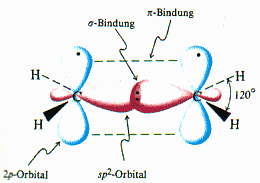
\includegraphics[width=0.5\textwidth]{pdfs/orbital.png}
\end{figure}

Eine exakte Beschreibung dieser Orbitale liegt der magnetischen Quantenzahl m
zugrunde. Bei der Überlagerung von zwei Orbitalen mit $m = 0$, spricht man
von einem $\sigma$-Orbital. Bei zwei $|m| = 1$ Orbitalen hingegen von $\pi$
Orbitalen.
\\
Mit der Hauptquantenzahl werden hier auch Elektronen unterschiedlicher
Energie im selben Orbital unterschieden, wobei wir hier die $1\sigma_y$ und
die 1s Zustände nicht untersuchen können, da diesen eine konstante
Druckverteilung im Resonator entspricht und diesem eine Resonanzfrequenz von 0
Hz entspricht.
\\
Bei der Überlagerung von zwei Orbitalen mit Hauptquantenzahl $n = 2$
entstehen zum einen $σ$- als auch $π$-Orbitale. Auch dort gibt es wieder
bindende- und antibindende-Orbitale.

\subsection{1-dimensionaler Festkörper}
Die theoretische Betrachtung des 1-dimensionalen Festkörpers in der klassischen Physik erfolgt über eine Kette aus durch Federn gekoppelten Massen.
Der folgende Abschnitt stammt aus der Festkörperphysikvorlesung von Prof.~Cinchetti im Wintersemester 2018/19.
Greift man sich eine Masse $n$ aus dieser Kette folgt in \glname{Newton}{scher} Mechanik
\begin{align}
  F_n &= \sum_{p\neq0} c_p\left[u_n(t)-u_{n+p}(t)\right]
  \intertext{mit der Federkonstanten $c_p$ und der Position}
  x_n(t) &= n\cdot a + u_n(t)\:.
  \intertext{Die Bewegungsgleichung der Masse $n$ ist mit der Betrachtung nur der nächsten Nachbarn und der Annahme}
  c_p &=
  \begin{cases}
    \;\;c, \text{wenn}\:p > n\\
    -c, \text{wenn}\:p < n
  \end{cases}\\
  M\frac{\ud^2u_n(t)}{\ud t^2} &= -c \left[2u_n(t)-u_{n+1}(t)-u_{n-1}(t)\right]\:. \label{eqn:1dstart}
  \intertext{Mit dem Ansatz}
  u_n(t) &= A\cdot\me^{iωt}\me^{iqna}
  \shortintertext{folgt}
  ω &= 2\sqrt{\frac{c}{M}} \left|\sin\left(\frac{qa}{2}\right)\right|\:. \label{eqn:omega1a}
  \intertext{Bisher wurde ein einatomiger Festkörper betrachtet.
    Für einen Stoff mit alternierender zweiatomiger Basis beginnen wir mit der Gleichung \eqref{eqn:1dstart} zweimal, die Atomsorten werden erst getrennt betrachtet.
    $u$ und $v$ bezeichnen hier die unterschiedlichen Atome, $C_1$ und $C_2$ die ebenfalls alternierenden Bindungsstärken.}
    M\frac{\ud^2u_n(t)}{\ud t^2} &= C_1 \left(v_n-u_n\right) + C_2 \left(v_{n-1}-u_n\right) \\
    M\frac{\ud^2v_n(t)}{\ud t^2} &= C_1 \left(u_n-v_n\right) + C_2 \left(u_{n+1}-v_n\right)
    \intertext{Mit dem gleichen Ansatz wie oben, folgt das Gleichungssystem}
    M \frac{\ud^2}{\ud t^2} \begin{pmatrix}u_n \\v_n \\\end{pmatrix}
    &= \begin{pmatrix}
      C_1+C_2-Mω^2 & -\left(C_1+C_2\me^{-iqa}\right) \\
      -\left(C_1+C_2\me^{-iqa}\right) & C_1+C_2-Mω^2 \\
    \end{pmatrix} \begin{pmatrix}u_n \\v_n \\\end{pmatrix}
    \intertext{Dieses kann entkoppelt werden in dem die Determinante der Matrix gleich null gesetzt wird.
    Die Frequenzen $ω$ ergeben sich dann zu}
    ω^2 &= \frac{C_1+C_2}{M} \pm \frac{1}{M} \sqrt{(C_1+C_2)^2-4C_1C_2\sin^2\left(qa\right)}\:.
\end{align}

\section{Durchführung}
\label{sec:Durchführung}

Der Versuchsaufbau besteht aus einer Drehschieberpumpe zur Erzeugung des Vakuums und dazugehörigem Vakuumbehälter.
In diesem Behälter befindet sich die eigentliche Messapperatur.
Diese ist in Abbildung \ref{fig:aufbau} dargestellt.
Die Einheiten sind jeweils $\si{\milli\meter}$ für alle Längen.
Die \alphat~werden, nach dem Austritt aus der Quelle, im Kollimator parallel ausgerichtet.
Anschließend streuen sie an einer dünnen Folie, im Laufe des Versuches werden verschiedene Materialien und Dicken verwendet.

\begin{figure}[ht]
  \centering
  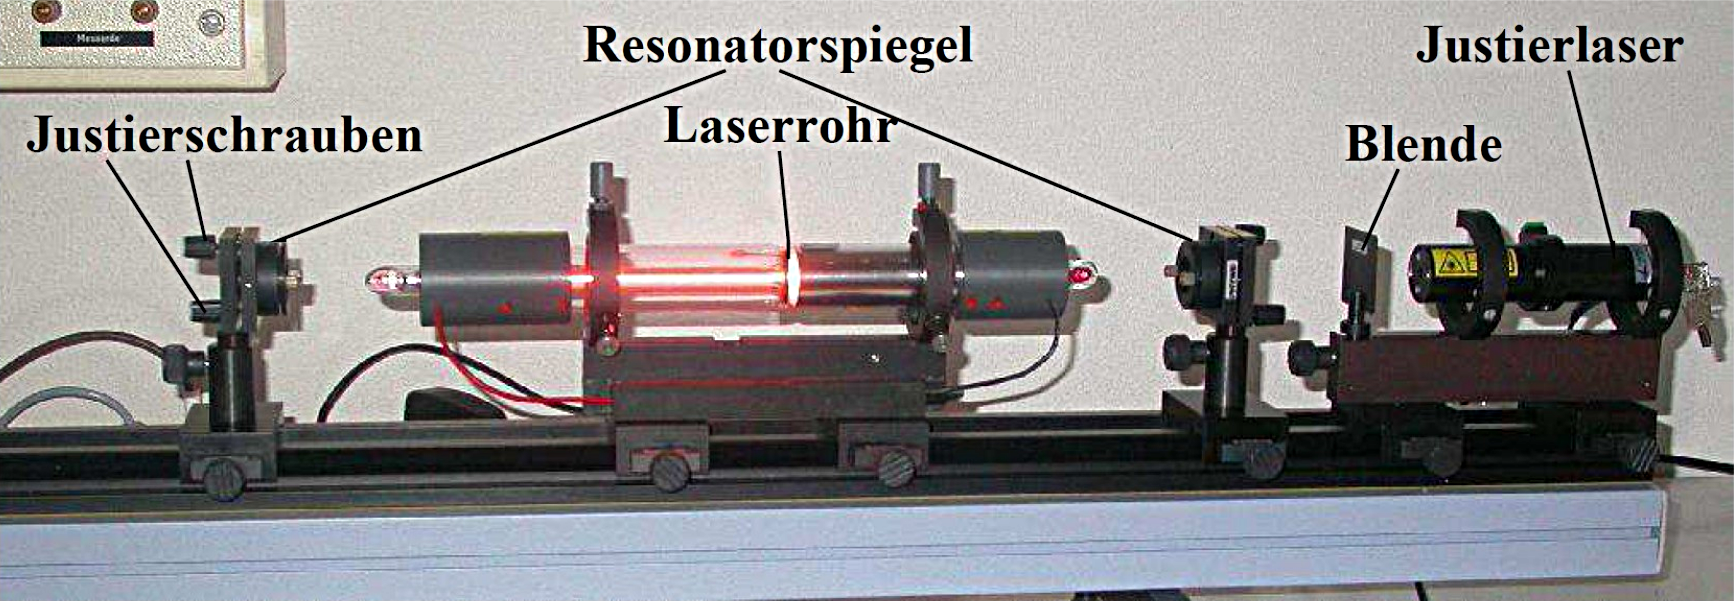
\includegraphics[width=0.8\textwidth]{images/aufbau.png}
  \caption{Skizze der Messapperatur. Längenangaben in Millimetern. \cite{anleitung}}
  \label{fig:aufbau}
\end{figure}

Der SB-Detektor kann um die Folie gedreht werden.
Die Stellung in Abbildung~\ref{fig:aufbau} entspricht $φ=\SI{0}{\degree}$.
Die Spannung des SB-Detektors bleibt während aller Messungen bei
$U_\text{det} = \SI{12}{\volt}$.

Das Ausgangsignal wird je nach Messung mit einem Oszilloskop dargestellt oder in einem Zählwerk detektiert.

In der ersten Messungen werden die Pulse des Detektors auf dem Oszilloskop zeitlich aufgelöst beobachtet.
Zuerst die unverstärkten und dann die, durch dem Zähler vorgeschaltetem Verstärker, verstärkten.

Der Einfluss der Foliendicke auf die Zählrate, in Kombination mit dem Kammerdruck, wird in der zweiten Messung bestimmt.
Hierfür wird die Impulshöhe auf dem Oszilloskop im Bereich von $\SI{0.04}{\milli\bar}$ bis $\SI{200}{\milli\bar}$ notiert.
Jeweils eine Messreihe für eine $\SI{2}{\micro\meter}$ Goldfolie und eine Messreihe ohne Folie.
Da die Impulshöhen schwanken wird eine maximale und minimale Amplitude genommen.

Die Winkelabhängigkeit der Zählrate wird, im Vakuum, für die 2 und $\SI{4}{\micro\meter}$ Goldfolie bestimmt.
Die Integrationszeit wird so gewählt, dass die Zählung ungefähr ein Ergebnis von $\num{1111}$ bringt.

Die Messung Nummer vier erfolgt zur Bestimmung des Einflusses von Mehrfachstreuungen.
Es wird bei einem festen Winkel für verschiedene Foliendicken die Anzahl an gestreuten Teilchen gemessen.

In der letzten Messung wird das Material der Folie geändert.
Bei einem Winkel von $\SI{20.1}{\degree}$ werden die Folien in Tabelle \ref{tab:folien}, bei einer Integrationszeit von
$\SI{300}{\second}$, verwendet:
\begin{table}
  \centering
  \caption{Verwendete Folien für die Z-Abhängigkeit.}
  \label{tab:folien}
  \begin{tabular}{c S[table-format=1.0]}
    \toprule
    {Material} & {Foliendicke$\:/\:\si{\micro\meter}$} \\
    \midrule
    Gold      & 4 \\
    Aluminium & 3 \\
    Bismut    & 2 \\
    \bottomrule
  \end{tabular}
\end{table}

\section{Auswertung}
\label{sec:Auswertung}
%\rot{
%  Sweep und Horizontal sind vertauscht gewesen. \\
%  Horizontal max 1A, → 1 Drehung 0,1A \\
%  Sweep max 3A → 1 Drehung 0,3A
%}

\subsection{Erdmagnetfeld}
Die Kompensation des Erdmagnetfeldes mit der Vertikalspule führt zu
einem Spulenstrom von $\SI{0.215}{\ampere}$.
Daraus ergibt sich mit den Daten in Tabelle \ref{tab:spulen}
und Gleichung \eqref{eqn:helmholtz}
\begin{equation}
  B_\text{V} = \left(\frac{4}{5}\right)^{\!\!\frac{3}{2}}
    \frac{μ_0 \cdot 20 \cdot \SI{0.215}{\ampere}}{\SI{11.735}{\centi\meter}}
  = \input{build/messung-b.tex}
\end{equation}
für die Vertikalkomponente des Erdmagnetfeldes.
Der Literaturwert \cite{erdmagnetfeld} beträgt
\begin{equation}
  B_\text{lit} = \SI{45.136}{\micro\tesla}\,.
\end{equation}

\subsection{Kernspins über die Resonanzen}
\label{sec:5.2}
Die Messwerte sind in Tabelle \ref{tab:messung-c} aufgetragen.
Von diesen ausgehend wird mit der Skalierung des Potentiometers von 0,3 multipliziert.
Die errechneten Stromstärken werden dann mit der Gleichung \eqref{eqn:helmholtz}
in die entsprechenden B-Feldstärken umgerechnet.
In der Abbildung \ref{fig:messung-c} sind diese gegen die Frequenz der Sinuswelle aufgetragen.

Die Bezeichung erfolgt anhand von Abbildung \ref{fig:messung-c-oszi} von links nach rechts.

Mit der Ausgleichsgeraden
\begin{equation}
  B_i = m_i \cdot f + b_i
\end{equation}
liefert \texttt{scipy} die Werte
\begin{align}
  \input{build/messung-c-m1.tex} \\
  \input{build/messung-c-b1.tex} \\
  \input{build/messung-c-m2.tex} \\
  \input{build/messung-c-b2.tex} \\
  \input{build/messung-c-m3.tex} \\
  \input{build/messung-c-b3.tex}\,.
\end{align}
Nach Gleichung \eqref{eqn:B_M_Theorie} sind die $m_i$
die Proportionalitätsfaktoren zwischen $f$ und $B$.
Mit umstellen zu
\begin{equation}
  g_{(f,i)} = \frac{4 \mpi \cdot \symup{m}_{\me}}{\me \cdot m_i}
\end{equation}
folgen die Werte
\begin{align}
  \input{build/messung-c-gf2.tex} \\
  \input{build/messung-c-gf3.tex}\,.
\end{align}
Mit der Gleichung
\begin{equation}
  I = \frac{g_j}{(4 \cdot g_3} - 1 +
    \sqrt{\left(\frac{g_j}{4 \cdot g_f} -1\right)^{\!\!2} + \frac{3}{4}
      \cdot \left(\frac{g_j}{g_f} -1\right)}
\end{equation}
ergeben sich die Kernspins zu
\begin{align}
  \input{build/messung-c-i2.tex} \\
  \input{build/messung-c-i3.tex}\,.
\end{align}
Durch einen Vergleich mit der Literatur \cite{opticalpumping} kann
das Minimum 2 $^{87}\text{Rb}$ mit einem Kernspin von $\sfrac{3}{2}$
und das Minimum 3 $^{85}\text{Rb}$ mit einem Kernspin von $\sfrac{5}{2}$
zugeordnet werden.

\begin{figure}
  \centering
  \includegraphics[width=0.8\textwidth]{build/messung-c.pdf}
  \caption{Darstellung der Daten aus Messung c).}
  \label{fig:messung-c}
\end{figure}

\begin{figure}
  \centering
  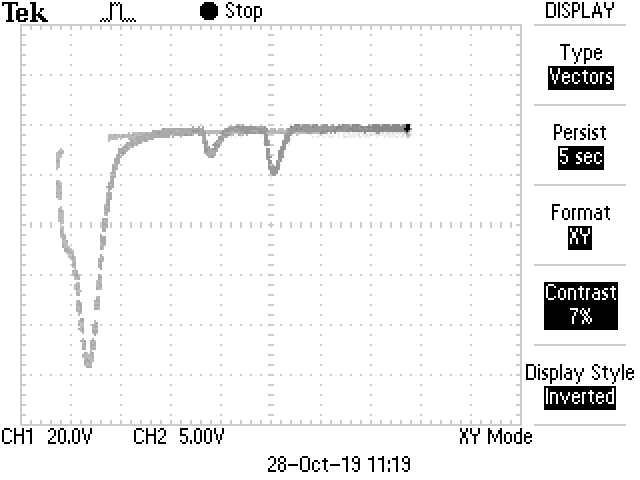
\includegraphics[width=0.8\textwidth]{data/messung-f/f1.JPG}
  \caption{Oszilloskopbild der Messung. (Messauftrag f)\newline
  Von links nach rechts: Min. 1 → Min. 2 → Min. 3}
  \label{fig:messung-c-oszi}
\end{figure}

\begin{table}
  \centering
  \caption{Messwerte und Magnetfeldstärken in der Messung c).}
  \label{tab:messung-c}
  \sisetup{table-format=1.2}
  \begin{tabular}{S[table-format=4.0] S[table-format=1.3] S S S[table-format=2.2] S S[table-format=2.2]}
    \toprule
    & \multicolumn{2}{c}{Minimum 1} & \multicolumn{2}{c}{Minimum 2}& \multicolumn{2}{c}{Minimum 3} \\
    {$f\:/\:\si{\kilo\hertz}$}
    & {$I_1\:/\:\si{\ampere}$} & {$B_1\:/\:\si{\micro\tesla}$}
    & {$I_2\:/\:\si{\ampere}$} & {$B_2\:/\:\si{\micro\tesla}$}
    & {$I_3\:/\:\si{\ampere}$} & {$B_3\:/\:\si{\micro\tesla}$} \\
    \midrule
     100 & 0.024 & 21.05 & 0.040 &  35.08 & 0.049 &  42.97 \\
     200 & 0.024 & 21.05 & 0.057 &  49.99 & 0.074 &  64.90 \\
     300 & 0.024 & 21.05 & 0.074 &  64.90 & 0.099 &  86.82 \\
     400 & 0.024 & 21.05 & 0.094 &  82.43 & 0.125 & 109.62 \\
     500 & 0.024 & 21.05 & 0.108 &  94.71 & 0.150 & 131.55 \\
     600 & 0.024 & 21.05 & 0.125 & 109.62 & 0.175 & 153.47 \\
     700 & 0.024 & 21.05 & 0.142 & 124.53 & 0.200 & 175.39 \\
     800 & 0.024 & 21.05 & 0.158 & 138.56 & 0.226 & 198.19 \\
     900 & 0.024 & 21.05 & 0.175 & 153.47 & 0.251 & 220.12 \\
    1000 & 0.024 & 21.05 & 0.193 & 169.25 & 0.276 & 242.04 \\
    \bottomrule
  \end{tabular}
\end{table}
\FloatBarrier
\subsection{Isotopenverhältnis}
Das Verhältnis wird über die Stärke der Pulse ermittelt,
dieses beträgt
\begin{equation}
  \frac{7}{11} = 0,\overline{63}\,,\quad\text{bzw.}\quad\frac{11}{7} = 1,57
\end{equation}
Es ergibt sich für die relativen Anteile
\begin{align}
  ^{87}\text{Rb}\!:\quad&\SI{39}{\percent} \\
  ^{85}\text{Rb}\!:\quad&\SI{61}{\percent}\,.
\end{align}
Die Literaturwerte \cite{opticalpumping} sind
\begin{align}
  ^{87}\text{Rb}\!:\quad&\SI{28}{\percent} \\
  ^{85}\text{Rb}\!:\quad&\SI{72}{\percent}\,.
\end{align}

\subsection{Quadratischer Zeeman-Effekt}
Nach Gleichung \eqref{eqn:zeequadr} kann der quadratische Zeeman-Effekt zu
\begin{align}
  \laplace E_{85} &= \SI{2.01e-24}{\joule} &\input{build/messung-h-dE3.tex} \\
  \laplace E_{87} &= \SI{4.53e-24}{\joule} &\input{build/messung-h-dE2.tex}
\end{align}
bestimmt werden.

\subsection{Schwing-Kernspin}
Die Funktion
\begin{equation}
  T = a + \frac{b}{x - c}
\end{equation}
wird, wieder mit \texttt{scipy} an die genommenen Messwerte gefittet.
Dabei ist $x$ die RF-Amplitude.
Die Parameter sind für die blaue Kurve
\begin{align}
  \input{build/messung-i-a1.tex} \\
  \input{build/messung-i-b1.tex} \\
  \input{build/messung-i-c1.tex}
  \intertext{und für die grüne Kurve}
  \input{build/messung-i-a2.tex} \\
  \input{build/messung-i-b2.tex} \\
  \input{build/messung-i-c2.tex}\,.
\end{align}
Das Verhältnis der Parameter $b_i$ beträgt
\begin{align}
  \frac{b_2}{b_1} &= \input{build/messung-i-bb.tex}\,,
  \intertext{der Literaturwert \cite{anleitung} ist}
  \frac{b_2}{b_1} &= 1,5\,.
\end{align}
\begin{figure}[ht]
  \centering
  \includegraphics[width=0.8\textwidth]{build/messung-i.pdf}
  \caption{Messwerte der Abschwingvorgänge.}
  \label{fig:messung-i.pdf}
\end{figure}

\FloatBarrier

\newpage
\section{Diskussion}
\label{sec:Diskussion}
Während der Messung lagen die Temperaturen von Gehäuse und Probe in dem
vorgegebenen Differenzbereich, wie in Abbildung \ref{fig:temperatur} gut zu sehen ist.
Außerdem wurde im vorgegebenen Rahmen geheizt.

Die Auffälligkeiten der Wärmekapazitäten $C_P$ und $C_V$ passen mit dem Verlauf
der Temperaturkurve zusammen, so mussten teilweise, wie in den Messwerten zu sehen ist,
die Ströme angepasst werden, was in der Temperaturkurve zu sehen ist und dann auch in den
Plots von $C_P$ \ref{fig:cp1} und $C_V$ \ref{fig:cv1}.

Bei der Bestimmung der \textsc{Debye}-Temperatur $Θ_D$ ist der Fehler dadurch gegeben,
dass die bestimmten $C_V$ Werte teilweise zwischen den Einträgen in der
gegebenen Tabelle liegen und hier die Übertragung Ungenauigkeiten reinbringt.

Die \textsc{Debye}-Temperatur liegt nach \cite{debye-copper} im Bereich
$310 - \SI{347}{\kelvin}$. Das experimentelle Ergebnis liegt darunter, was an
der Tabelle liegen kann, das berechnete in dem Intervall.

%\newpage
\printbibliography{}
\includepdf[pages=-]{data/messwerte1.PDF}
\includepdf[pages=-]{data/messwerte2.PDF}

\begin{table}
  \centering
  \caption{Neue Messwerte $\text{TEM}_{10}$.}
  \label{tab:tem10-neu}
  \begin{tabular}{S[table-format=2.1] S[table-format=3.0]
                  S[table-format=1.1] S[table-format=2.0]
                  S[table-format=2.1] S[table-format=2.0]
                  S[table-format=2.1] S[table-format=2.0]}
    \toprule
    {$\text{Diode}\;/\;\si{\milli\meter}$} & {$I\;/\;\si{\nano\ampere}$} &
    {$\text{Diode}\;/\;\si{\milli\meter}$} & {$I\;/\;\si{\nano\ampere}$} &
    {$\text{Diode}\;/\;\si{\milli\meter}$} & {$I\;/\;\si{\nano\ampere}$} &
    {$\text{Diode}\;/\;\si{\milli\meter}$} & {$I\;/\;\si{\nano\ampere}$} \\
    \midrule
    -15.0 &  34 & -1.0 & 65 &  7.0 & 10 & 15.0 & 91 \\
    -14.0 &  40 & -0.5 & 56 &  7.5 & 12 & 16.0 & 95 \\
    -13.0 &  77 &  0.0 & 48 &  8.0 & 14 & 17.0 & 93 \\
    -12.0 &  85 &  0.5 & 43 &  8.5 & 18 & 18.0 & 90 \\
    -11.0 & 103 &  1.0 & 34 &  9.0 & 20 & 19.0 & 82 \\
    -10.0 & 110 &  1.5 & 28 &  9.5 & 22 & 20.0 & 74 \\
     -9.0 & 120 &  2.0 & 22 & 10.0 & 27 & 21.0 & 67 \\
     -8.0 & 135 &  2.5 & 16 & 10.5 & 31 & 22.0 & 55 \\
     -7.0 & 137 &  3.0 & 11 & 11.0 & 37 & 23.0 & 57 \\
     -6.0 & 130 &  3.5 &  8 & 11.5 & 40 & 24.0 & 53 \\
     -5.0 & 125 &  4.0 &  3 & 12.0 & 48 & 25.0 & 50 \\
     -4.0 & 120 &  4.5 &  1 & 12.5 & 53 & 26.0 & 40 \\
     -3.0 & 100 &  5.0 &  2 & 13.0 & 60 & 27.0 & 33 \\
     -2.5 & 100 &  5.5 &  3 & 13.5 & 67 & 28.0 & 26 \\
     -2.0 &  92 &  6.0 &  4 & 14.0 & 73 & 29.0 & 16 \\
     -1.5 &  80 &  6.5 &  7 & 14.5 & 80 & 30.0 & 11 \\
    \bottomrule
  \end{tabular}
\end{table}
\end{document}
